

\chapter{Towards an improved specification for capitalization tables based on the Open Cap Table format}\label{ch:towards}

\section{Requirements of a consistent model for capitalization tables}

A consistent model for \glspl{capitalization-table} should be able to guarantee that the following requirements hold:

\begin{itemize}
	\item The total number of shares in circulation must never exceed the number of shares issued by the issuer.
	\item \Glspl{issuance} create new shares, transfers do not create new shares, cancellations destroy shares.
	      \begin{itemize}
		      \item Cancellations and transfers fully consume their input security. A balance \gls{security} is created in case of partial cancellations or transfers
		      \item Securities must either be issued or be a result or balance \gls{security} of a transfer or the balance \gls{security} of a cancellation
	      \end{itemize}
	\item Every \gls{security} is owned by one and only one \gls{stakeholder}
	\item Every \gls{security} can be traced back to a single \gls{issuance}.
	\item Every \gls{security} in a \gls{stakeholder}'s portfolio can be traced back to the transaction that issued it to the \gls{stakeholder} or that transferred it to the \gls{stakeholder}
\end{itemize}

There is nothing exceptional about these requirements.

They are naturally expected in the accounting and finance domain. However, they are not enforced by the Open Cap Table format, and could not be, given the limitations of JSON Schema.

\section{Expressiveness of the contracts and vesting rules}

The greatest complexity in validating the transactions that compose a \gls{capitalization-table} lies in employee stock option plans. Stock options awarded to employees are subject to vesting rules, which are usually complex and vary from company to company.

The variety of vesting rules that can be found in actual stock option grants are written in legal documents, and limited only by the creativity of lawyers.

Therefore, a model for \glspl{capitalization-table} should be able to express a range of vesting rules. The vesting rules that can be expressed by the Open Cap Table format can be improved simply by adding a propositional logic layer to the vesting rules.

\section{An introduction to Alloy}

Alloy, first introduced by Daniel Jackson in 2002~\cite{jackson-2002}, is today a complete framework for modeling and analyzing software systems. We say it is a framework because it is composed of more than just a modeling language.

The idea underlying Alloy is that ``software should be built on abstractions'', and that by picking the right ones, programming should ``naturally from design''.

Alloy is distributed as the Alloy Analyzer, which features:

\begin{itemize}
	\item A modeling language
	\item A visualizer for metamodels and model instances
	\item A bounded model checker
	\item A standard library for common data structures (sequences, graphs, relations, etc.)
\end{itemize}

By combining the three features above, an Alloy user can quickly iterate on a model, visualize and explore instances, and express and check properties. An Alloy model can focus both on the concepts underneath the system being modeled, on the data model and relationships, and on more operational aspects of the system by modeling relations between two or more states.

\subsection{Parts of an Alloy model}

Every alloy model is composed of signatures, predicates, facts, functions, assertions, and commands:

\begin{enumerate}
	\item Signatures: the basic building blocks of Alloy models, they represent entities in the domain. Signatures have \textit{fields} that relate them to other signatures.
	\item Functions: A function in Alloy relates instances of signatures to relations. An alloy function is a function like in any programming language.
	\item Predicates: A predicate in Alloy is a function that returns a boolean value. Predicates are used to express properties of the model.
	\item Facts: A fact is a predicate that must always be true in the model. A fact actively constrains the model by discarding instances that do not satisfy it.
	\item Assertions: An assertion is a predicate that can be given to a check command, and expresses our \textit{expectations} of the model. Assertions do not constrain the model effectively.
	\item Commands (Checks and runs): The \verb|run| finds \textit{examples} of the model that satisfy all constraints, while the \verb|check| command finds \textit{counter-examples} that violate a given assertion.
\end{enumerate}

To illustrate the concepts above, we give a very model and analyze its parts.

\begin{listing}[H]
\begin{minted}{alloy}
sig Stakeholder {
    portfolio : set Security
}

sig Security {
    owner : one Stakeholder
}

fact invOwnerPort { ~owner = portfolio }

pred overlap[s1, s2 : Stakeholder] {
    s1.portfolio & s2.portfolio != none
}

assert noSharedOwnership {
    no disj s1, s2 : Stakeholder | overlap[s1, s2]
}
\end{minted}
\caption{A simple Alloy model}
\label{lst:alloy-model}
\end{listing}

In our case, there are signatures for two concepts in our domain: \glspl{security} and stakeholders, which own \glspl{security} by having a portfolio.

We can note that Alloy gives more control over the cardinality of relationships than a class or table: \verb|portfolio| is a set of \verb|Security|, and not a single \verb|Security|.

The fact states that \verb|owner| and \verb|portfolio| are inverses of each other (their union forms a symmetrical relation), which is a constraint that must always hold in the model. Alloy uses the \verb|~| operator to denote the inverse of a relation.

The predicate \verb|overlap| tells us whether two different \glspl{stakeholder} can any \gls{security} in common in the portfolio, which we would not expect in a real-world scenario.

The \verb|noSharedOwnership| assertion tells us that there are no two \glspl{stakeholder} that own the same security.

\subsection{Using the Alloy Analyzer}

The user can analyze an Alloy model by checking whether certain assertions hold, or by running simulations of instances of the model. Alloy can find counterexamples to assertions, and can also find instances that satisfy certain properties.

We can ask Alloy to check whether the assertion \verb|noSharedOwnership| holds by issuing a check command (for a scope of size 5):

\begin{listing}
	\begin{minted}{alloy}
		check noSharedOwnership for 5
	\end{minted}
	\caption{Checking an assertion}
	\label{lst:alloy-check}
\end{listing}

We explicitly ask Alloy to use a scope of 5, meaning there will be at most 5 stakeholders, 5 \glspl{security}.  It is essential to bounded-model checking to give a bound.

After a few tenths of a second, Alloy will tell us that the assertion holds, by stating that it couldn't find a counterexample:

\begin{listing}\label{lst:alloy-check-output}
	\begin{verbatim}
Executing "Check noSharedOwnership for 5"
Solver=minisatprover(jni) 
    Bitwidth=4 MaxSeq=5 
    SkolemDepth=4 Symmetry=20 Mode=batch
Generating CNF...
820 vars. 70 primary vars. 1280 clauses. 193ms.
Solving...
No counterexample found. Assertion may be valid. 16ms.
core reduced from 8 to 6 top-level formulas. 138ms.
\end{verbatim}
	\caption{Alloy's output}
\end{listing}

\newpage

Finally, we can issue a \verb|run| command to find instances of the model that satisfy the constraints:

\begin{listing}[H]\label{lst:alloy-run}
	\begin{minted}{alloy}
run {} for 5 but exactly 2 Stakeholder, 5 Security
\end{minted}
	\caption{Running the model}
\end{listing}

A sample visualization generated by the run command is show below in figure~\ref{fig:alloy-run}.

\begin{figure}[H]
	\centering
	\fbox{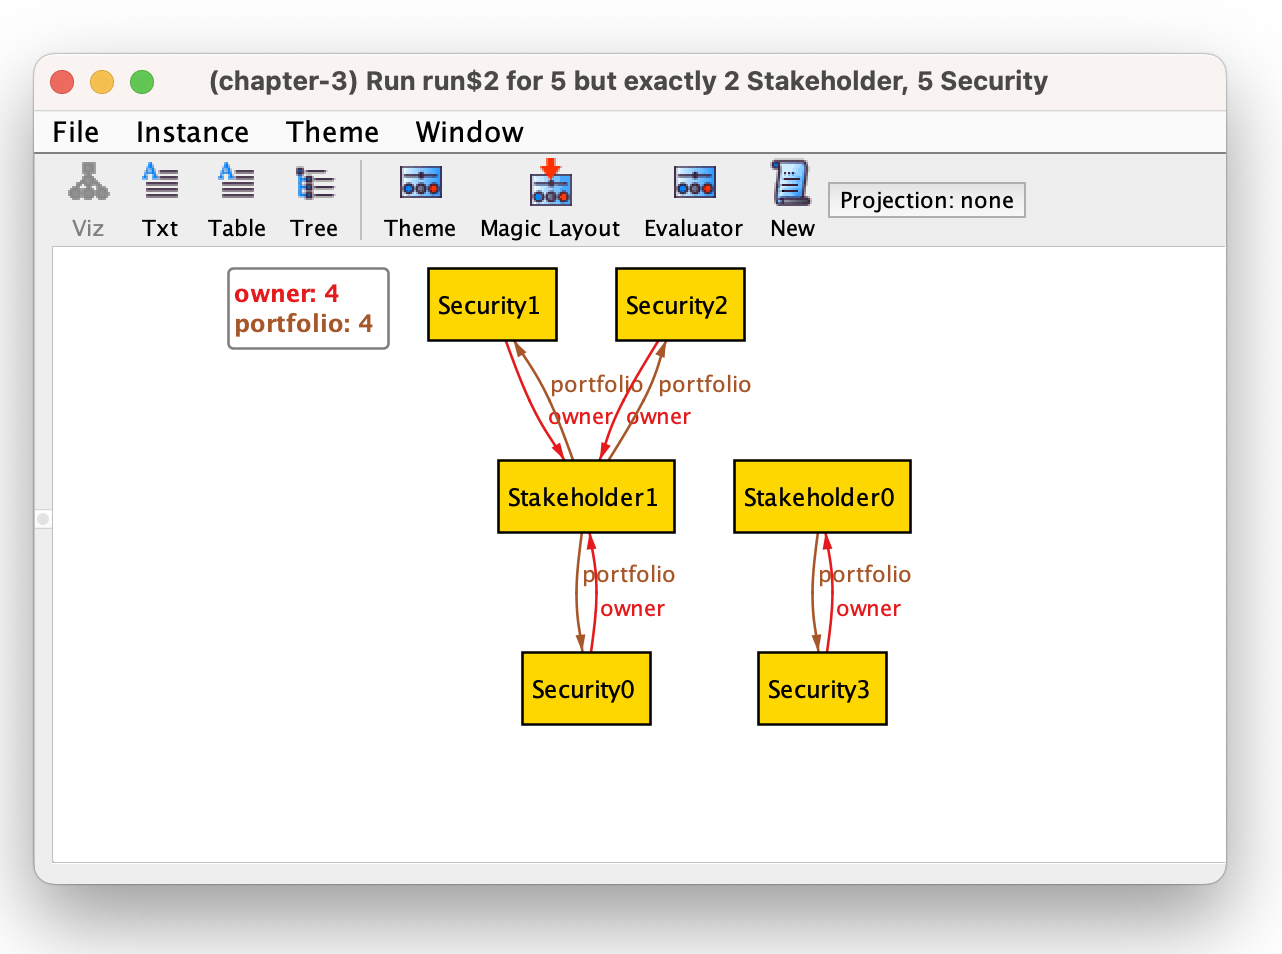
\includegraphics[width=0.8\textwidth]{images/alloy-run.png}}
	\caption{A sample instance generated by Alloy}\label{fig:alloy-run}
\end{figure}

\subsection{Refining a model}

We know the model is correct (up to a bound). But why? We can use Alloy to find out.

\newpage

The technique is to turn the \verb|invOwnerPort| fact into a \textit{predicate}; meaning that we do not assume it holds. But we can still ask Alloy to check whether it \textit{suffices} for \verb|noSharedOwnership| to hold, with a small change in the model:

\begin{listing}[H]\label{lst:alloy-strengthen}
	\begin{minted}{alloy}
pred invOwnerPort { ~owner = portfolio }
\end{minted}
	\caption{Strengthening the model}
\end{listing}

Now, the \verb|noSharedOwnership| assertion does not hold anymore, since we can find a counterexample:

\begin{listing}[H]\label{lst:alloy-strengthen-output}
	\begin{verbatim}
Executing "Check noSharedOwnership for 5"
Solver=minisatprover(jni) 
    Bitwidth=4 MaxSeq=5 
    SkolemDepth=4 Symmetry=20 Mode=batch
Generating CNF...
767 vars. 70 primary vars. 1177 clauses. 85ms.
Solving...
Counterexample found. Assertion is invalid. 14ms.
\end{verbatim}
	\caption{Alloy's output with a counterexample after strengthening the model}
\end{listing}

We call \verb|check| with a modified assertion, namely:

\begin{listing}[H]\label{lst:alloy-strengthen-check}
	\begin{minted}{alloy}
check noSharedOwnershipAlt {
    invOwnerPortfolio implies {
        no disj s1, s2 : Stakeholder | overlap
    }
}
\end{minted}
	\caption{Checking the model again, considering the strengthened assumptions}
\end{listing}

\newpage

Now we see that the model is still correct. That holds, but only because of the \verb|invOwnerPortfolio| predicate:

\begin{listing}[H]\label{lst:alloy-strengthen-check-output}
	\begin{verbatim}
Executing "Check noSharedOwnershipAlt"
Solver=minisatprover(jni) 
    Bitwidth=4 MaxSeq=4 
    SkolemDepth=4 Symmetry=20 Mode=batch
Generating CNF...
318 vars. 30 primary vars. 476 clauses. 104ms.
Solving...
No counterexample found. Assertion may be valid. 6ms.
core reduced from 8 to 6 top-level formulas. 23ms.
\end{verbatim}
	\caption{Alloy's output showing no counterexample after considering the strengthened assumptions}
\end{listing}

There is much going on underneath Alloy to make this possible, ultimately relying on the KodKod library~\cite{TorlakJackson2007} to translate Alloy problems to and from SAT problems.

A full presentation of Alloy is beyond the scope of this work, but can be found in the Software Abstractions book by Daniel Jackson~\cite{jackson-2012}.

\section{From JSON Schema to Alloy}

The OCF is chiefly a data format, while we are looking for a conceptual model. Nevertheless, the OCF is a good starting point for a conceptual model, and we can use it to derive a conceptual model that is more expressive and that can be used to validate capitalization tables.

The general approach has the following steps:

\begin{enumerate}
	\item Define the signatures roughly matching the documents in the JSON Schema, even if we must declare them as abstract before refining them
	\item Refine the signatures by adding fields and constraints, based on the keys and values in the JSON Schema
	\item Add expected properties (of the model) as assertions composed of predicates
	\item Check that assertions hold, or debug the model until they do
\end{enumerate}

Step 1 is very mechanical and straightforward. Step 2 requires some attention to detail, since relations in JSON schema are very different from those in Alloy. JSON Schema mostly defines JSON objects, which are associative maps. Some documents define an array of objects, or refer to other documents by ID.~On the other hand, Alloy provides fine-grained control over the arity and multiplicity of relations. Step 3 requires domain expertise and some training in the background relations, set and logic, and some creativity. Step 4 is a matter of running the Alloy Analyzer and checking the results, plus some debugging.

The whole process is not exceedingly difficult to perform, specially if compared to alternatives, Such as Z, TLA$^{+}$, or dependently typed languages and proof assistants such as Agda, Coq or Idris. It resembles writing SQL schemas or business domain entities in object-oriented languages, but it does require some familiarity with mathematics (set theory and logic).

\section{A brief overview of Alloy related literature}

Alloy is cited in more than 1,200 papers, with many extensions and applications
in software design and modeling. Alloy$\ast$ is a higher-order extension of
Alloy that can be used for program synthesis, since it supports higher-order
quantification~\cite{Milicevic2017}. $\alpha{Rb}y$ is an embedding of Alloy in
Ruby~\cite{Arby}.

A number of other modeling languages have been translated to or partially modeled in Alloy\cite{alloy-case-studies}, including UML, $i^\star$, CVL, Event-B and, Z, OCL.\@Alloy can also be used with verification languages such as ACL2 or Isabelle.

Alloy has been used in a wide range of applications in software engineering, database design, \gls{security} analysis~\cite{Carpio2021}\cite{Chen2006}, multiagent negotiations~\cite{Podorozhny}. It has also been applied to modeling beyond computer science, such as a model for central bank policy~\cite{Johnson2021}. A model of the same-origin-policy used in web browsers can be found in the 500 Lines or Less open-source book~\cite{500Lines19:online}.

\textit{We were unable to find previous models of \glspl{capitalization-table} in Alloy.}
